\subsection{Évaluation}
L’évaluation est constituée de vignettes à découper (fig.~\ref{bande}) et à coller sur la feuille d’évaluation (fig.~\ref{eval}, p.~\pageref{eval}). Le critère d’évaluation de la compétence \og Reconnaitre une étape du développement d’un végétal \fg{} est précisé à la table~\ref{criteres}.

\begin{figure}[h!tbp]
\centering
\noindent
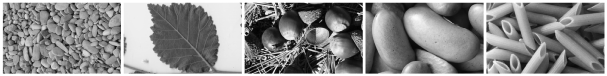
\includegraphics[width=\echelle\textwidth]{bande.png}
\caption{Vignettes à découper}
\label{bande}
\end{figure}

\begin{figure}[h!tbp]
\centering
\noindent
\fcolorbox{black}{white}{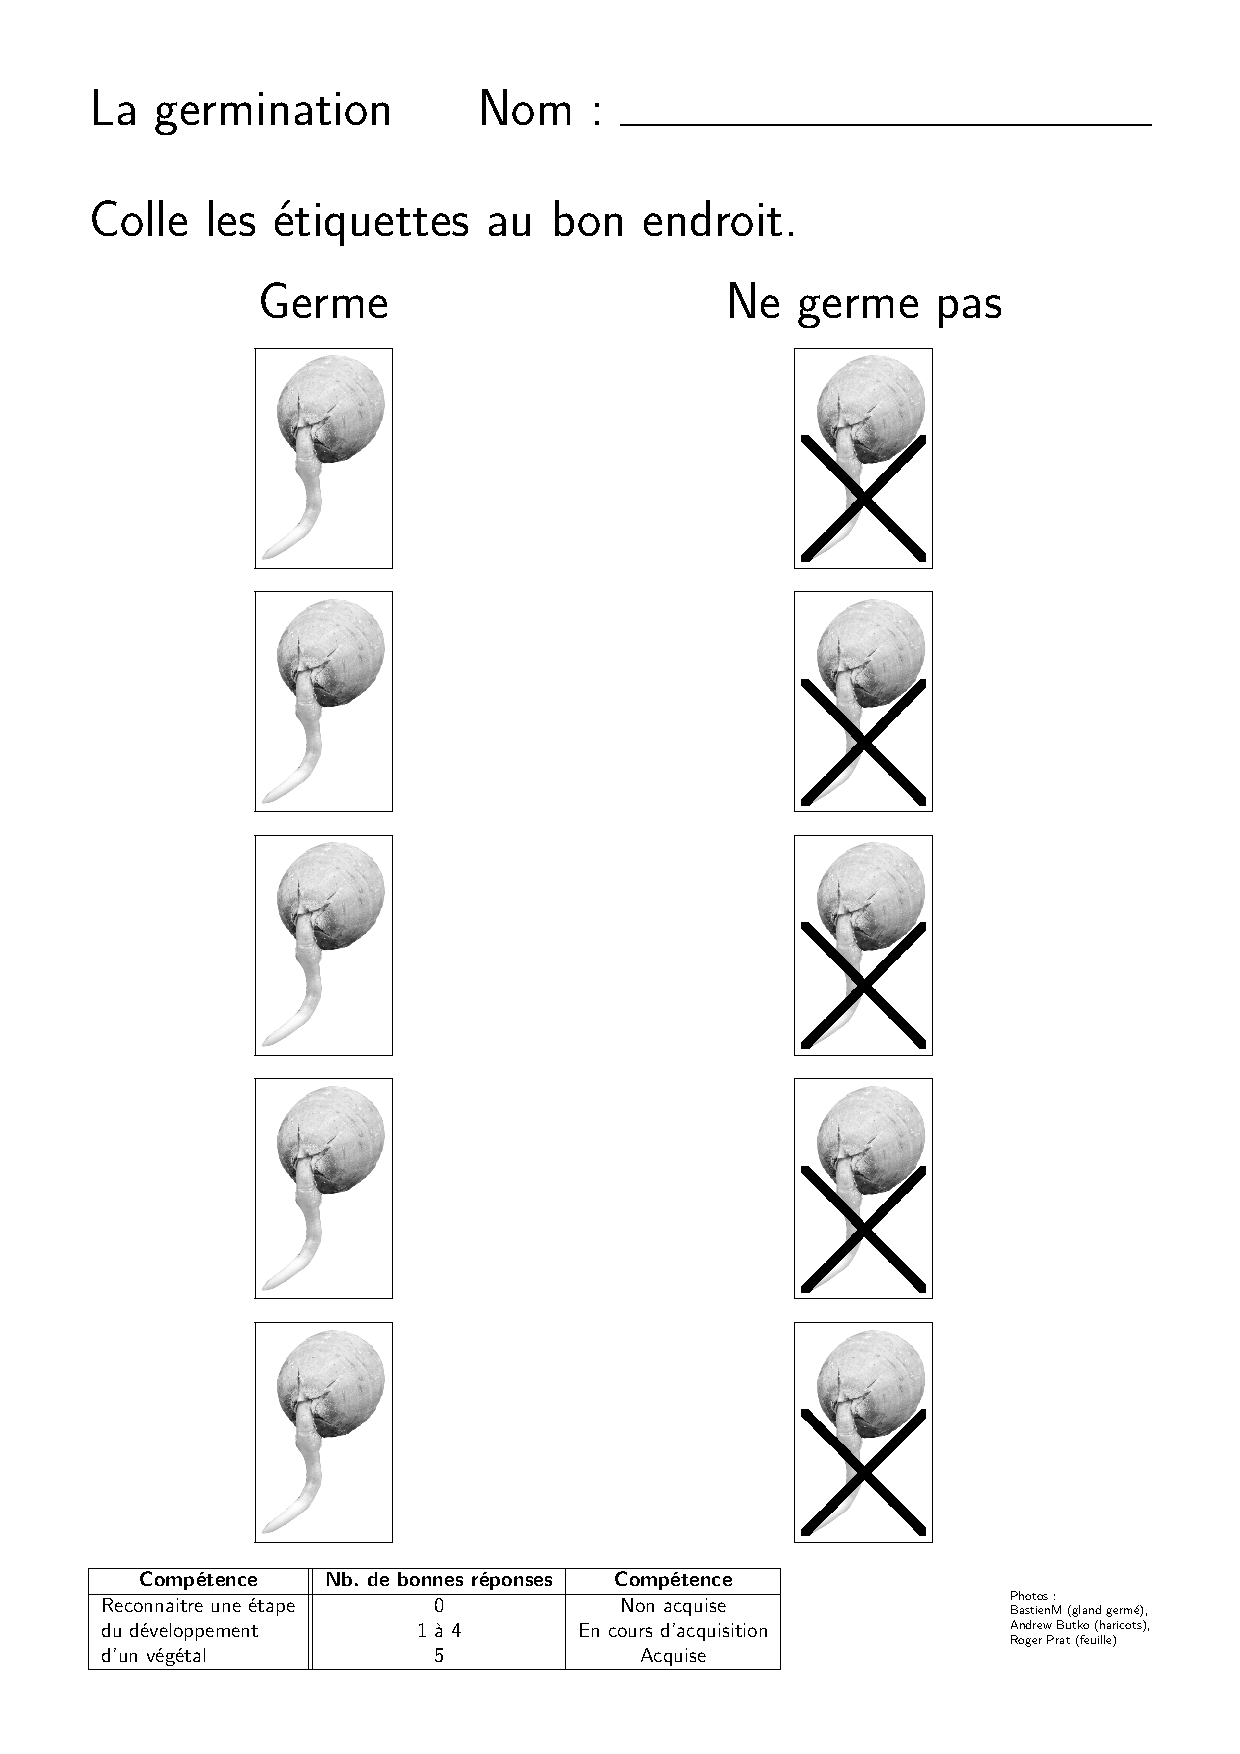
\includegraphics[width=\echelle\textwidth]{tex/eval.pdf}}
\caption{Feuille d’évaluation}
\label{eval}
\end{figure}

\setcounter{table}{0}
%\renewcommand\tablename{\textsc{Tableau}}
\begin{table}[h!tbp]
\centering
\begin{tabular}{|c|c|}
\hline 
\textbf{Nb. de bonnes réponses} & \textbf{Compétence} \\ 
\hline 
0 & Non acquise \\ 
1 à 4 & En cours d’acquisition \\
5 & Acquise \\ 
\hline 
\end{tabular}
\caption{\label{criteres} Critère d’évaluation}
\end{table}

\clearpage